%% LyX 2.3.6 created this file.  For more info, see http://www.lyx.org/.
%% Do not edit unless you really know what you are doing.
\documentclass[english]{article}
\usepackage[T1]{fontenc}
\usepackage[latin9]{inputenc}
\usepackage{float}
\usepackage{url}
\usepackage{amstext}
\usepackage{graphicx}

\makeatletter

%%%%%%%%%%%%%%%%%%%%%%%%%%%%%% LyX specific LaTeX commands.
%% Because html converters don't know tabularnewline
\providecommand{\tabularnewline}{\\}
\floatstyle{ruled}
\newfloat{algorithm}{tbp}{loa}
\providecommand{\algorithmname}{Algorithm}
\floatname{algorithm}{\protect\algorithmname}

\makeatother

\usepackage{babel}
\begin{document}
\title{A two phase evolutionary method to train RBF networks}
\author{Ioannis G. Tsoulos, Alexandros Tzallas, Evangelos Karvounis}
\date{Department of Informatics and Telecommunications, University of Ioannina,
Greece}
\maketitle
\begin{abstract}
This article proposes a two phase hybrid method to train RBF neural
networks for classification and regression problems. During the first
phase a range for the critical parameters of the RBF network is estimated
and in the second phase a genetic algorithm is incorporated to locate
the best RBF neural network for the underlying problem. The method
is compared against other training methods of RBF neural networks
on a wide series of classification and regression problems from the
relevant literature and the results are reported.
\end{abstract}
\begin{description}
\item [{Keywords:}] RBF networks, classification, regression, genetic algorithms.
\end{description}

\section{Introduction}

In machine learning appear many practical problems such as classification
and regression problems. A good programming tool that can be used
to tackle this problem is Radial Basis Function (RBF) networks\cite{rbf1}.
These networks typically are expressed as a function:\textbf{
\begin{equation}
y(x)=\sum_{i=1}^{k}w_{i}\phi\left(\left\Vert x-c_{i}\right\Vert \right)\label{eq:firstrbf}
\end{equation}
}where $\overrightarrow{x}$ is the input pattern, the vector $\overrightarrow{w}$
is called the weight vector and $y(x)$ is the predicted value of
the network. RBF networks are feedforward neural networks\cite{ann-bishop}
with three computational layers: 
\begin{enumerate}
\item The input layer, where the problem is presented in the form of patterns
to the neural network
\item The processing layer, where a computation is performed using the Gaussian
processing units $\phi(x)$. These units can have many forms in the
relevant literature but the most used form is the Gaussian function
expressed as: \textbf{
\begin{equation}
\phi(x)=\exp\left(-\frac{\left(x-c\right)^{2}}{\sigma^{2}}\right)
\end{equation}
}The value $\phi(x)$ depends only on the distance of vector $\overrightarrow{x}$
from some other vector $\overrightarrow{c}$, which typically is called
centroid. 
\item The output layer where the output of every function $\phi(x)$ is
multiplied by a corresponding weight value $w_{i}$.
\end{enumerate}
RBF networks have been used in many classification and regression
problems from the areas of physics \cite{rbfphysics1,rbfphysics2,rbfphysics3,rbfphysics4},
medicine \cite{rbfmed1,rbfmed2,rbfmed3},\textbf{ }solution of differential
equations\textbf{ }\cite{rbfde1,rbfde2}, chemistry \cite{rbfchemistry1,rbfchemistry2,rbfchemistry3},
economics \cite{rbfecon1,rbfecon2,rbfecon3}, digital communications
\cite{rbfnetwork1,rbfnetwork2}\textbf{ }etc. Also, recently the RBF
networks have been used in more difficult problems such as authentication
assurance of meat products \cite{rbf_add1}, trajectory tracking for
electro-hydraulic servo systems, identification of geographical origin
for foods \cite{rbf_add3}, prediction of solution gas-oil ratio of
crude oil systems \cite{rbf_add4}, prediction of occurrences of haloketones
in tap water \cite{rbf_add5} , health monitoring \cite{rbf_add6}
etc. Because of the extensive use of RBF networks, many methods have
been proposed in the recent literature to enhance them. There are
methods that parallelize the RBF networks \cite{rbfparallel,rbfgpu},
methods that improve the initialization of the RBF parameters\textbf{
}\cite{rbfinit1,rbfinit2,rbfinit3}, methods that alter the architecture
of the network\textbf{ }\cite{rbfprun1,rbfprun2,rbfprun3}, methods
aimed to locate the best set of the RBF parameters with global optimization
techniques\cite{rbfpso1,rbfpso2,rbfdiff1} etc. This article transforms
the problem of RBF training into an optimization problem and applies
a modified genetic algorithm technique to solve it. The global optimization
problem is defined as :
\begin{equation}
\min\left(E\left(y\right)\right)=\sum_{i=1}^{m}\left(y\left(x_{i}\right)-t_{i}\right)^{2}\label{eq:eqrbf}
\end{equation}
where $m$ is the total number of input patterns and $t_{i}$ is the
output for pattern $x_{i}$. The suggested approach has two phases:
firstly reasonable bounds for the RBF parameters are estimated using
the k-means \cite{kmeans} algorithm and in the second phase the modified
algorithm is used to solve the problem of equation \ref{eq:eqrbf}
inside the bounds located in the first phase.\textbf{ }

The rest of this paper is organized as follows: in section \ref{sec:Method-description}
the proposed method is described, in section \ref{sec:Experiments}
the conducted experiments are listed and the proposed method is compared
against the traditional training of RBF networks and finally in section
\ref{sec:Conclusions} some conclusions are derived.

\section{Method description\label{sec:Method-description}}

The proposed method can be divided into two main phases: during the
first phase an approximation for the bound of RBF parameters is made
using the K-Means algorithm in the second phase the optimization problem
is solved using a modified genetic algorithm. These phases are outlined
in detail in the following subsections.

\subsection{Bound location phase \label{subsec:Bound-location-phase}}

The proposed genetic algorithm has chromosomes with dimension $(d+1)\times k$,
where $d$ is the dimension of the input problem, i.e. the dimension
of the vector $\overrightarrow{x_{i}}$ in equation \ref{eq:eqrbf}
and $k$ is the total number of processing units of the RBF network.
The layout of each chromosome is presented in Figure \ref{fig:The-layout-of}.
Every center $\overrightarrow{c_{i}}$ in the equation \ref{eq:firstrbf}
is a vector of dimension $d$ and also an additional parameter is
reserved for the parameter $\sigma$ of every $\phi(x)$ function.
The centroids and the corresponding variances are estimated using
the k-means algorithm that described in algorithm \ref{alg:The-KMeans-algorithm.}.
The value $\sigma_{i}$ for every $\phi_{i}(x)$ is calculated as:
\begin{equation}
\sigma_{i}=\sum_{j=1}^{d}s_{ij}^{2}
\end{equation}
After the estimation of $c_{i}$ and $\sigma_{i}$ the vectors $\overrightarrow{L},\ \overrightarrow{R}$
with dimension $(d+1)\times k$ are constructed. These vectors will
serve as the bounds for the chromosomes of the genetic population.
These vector are constructed using the following procedure:
\begin{enumerate}
\item \textbf{Set} m=0
\item \textbf{Set} $F>1$ 
\item \textbf{For} $i=1..k$ \textbf{do}
\begin{enumerate}
\item \textbf{For} $j=1..d$ \textbf{do}
\begin{enumerate}
\item \textbf{Set} $L_{m}$=$-F\times c_{ij}$, $R_{m}$=$F\times c_{ij}$
\item \textbf{Set} $m=m+1$
\end{enumerate}
\item \textbf{EndFor}
\item \textbf{Set} $L_{m}=-F\times\sigma_{i}$, $R_{m}=F\times\sigma_{i}$
\item \textbf{Set} $m=m+1$
\end{enumerate}
\item \textbf{EndFor}
\end{enumerate}
\begin{figure}
\caption{The layout of the chromosomes in the proposed genetic algorithm.\label{fig:The-layout-of}}

\centering{}%
\begin{tabular}{|c|c|c|c|c|c|c|c|c|c|c|c|c|c|c|c|}
\hline 
$c_{11}$ & $c_{12}$ & ... & $c_{1d}$ & $\sigma_{1}$ & $c_{21}$ & $c_{22}$ & ... & $c_{2d}$ & $\sigma_{2}$ & ... & $c_{k1}$ & $c_{k2}$ & ... & $c_{kd}$ & $\sigma_{k}$\tabularnewline
\hline 
\end{tabular}
\end{figure}
\begin{algorithm}
\caption{The k-means algorithm.\label{alg:The-KMeans-algorithm.}}

\begin{enumerate}
\item \textbf{Repeat}
\begin{enumerate}
\item $S_{j}=\left\{ \right\} ,\ j=1..k$
\item \textbf{For} every sample $x_{i}$ \textbf{Do}
\begin{enumerate}
\item \textbf{Set} $j^{*}=\min_{i=1}^{k}\left\{ D\left(x_{i},c_{j}\right)\right\} $,
where $j^{*}$ is the nearest center for sample $x_{i}$. 
\item \textbf{Set} $S_{j^{*}}=S_{j^{*}}\cup\left\{ x_{i}\right\} $.
\end{enumerate}
\item \textbf{EndFor}
\item \textbf{For} every center $c_{j}$ \textbf{Do}
\begin{enumerate}
\item \textbf{Set} $M_{j}$=number of elements in $S_{j}$
\item \textbf{Update} $c_{j}$
\[
c_{j}=\frac{1}{M_{j}}\sum_{i=1}^{M_{j}}x_{i}
\]
\end{enumerate}
\item \textbf{EndFor} 
\end{enumerate}
\item \textbf{Calculate} the corresponding variances 
\[
s_{j}^{2}=\frac{\sum_{i=1}^{M_{j}}\left(x_{i}-c_{j}\right)^{2}}{M_{j}}
\]
\item \textbf{Terminate} when $c_{j}$ no longer change.
\end{enumerate}
\end{algorithm}


\subsection{Main algorithm }

The genetic algorithm used here is based on the algorithm denoted
as $\mbox{GA}\left(c_{r1},l\right)$ in the paper of Kaelo and Ali\cite{kaeloali}
 with a modified stopping rule as proposed in \cite{Tsoulos1}. The
basic steps of the main algorithm are given below:
\begin{enumerate}
\item \textbf{Initialization Step}
\begin{enumerate}
\item \textbf{Read} the train set with $m$ patterns of $d$ dimension. 
\item \textbf{Set} $k$ the number of nodes for the RBF network.
\item \textbf{Estimate} the vectors $\overrightarrow{L},\ \overrightarrow{R}$
using the procedure of subsection \ref{subsec:Bound-location-phase}. 
\item \textbf{Initialize} a genetic population of $N_{C}$ random chromosomes
inside $[L,R]$. 
\item \textbf{Set} the selection rate $p_{s}\in[0,1]$, the mutation rate
$p_{M}\in[0,1]$ , $iter=0,$ and $i_{max}$ the maximum number of
generations.
\end{enumerate}
\item \textbf{Evaluation Step}

\textbf{For} every chromosome $g$ \textbf{calculate} using the procedure
defined in subsection \ref{subsec:Fitness-evaluation} the fitness
$f_{g}$.
\item \textbf{Genetic operations step}\\
During this step three genetic operations are performed: selection,
crossover and mutation.
\begin{enumerate}
\item \textbf{Selection procedure.} Firstly the chromosomes are sorted with
relevance to their corresponding fitness value. The best $\left(1-p_{s}\right)\times N_{c}$
are transferred without change to the next generation and the remain
ones are substituted by offsprings created through the crossover procedure.
In the crossover procedure the mating parent are selected using tournament
selection for every parent. The tournament selection has as follows: 
\begin{enumerate}
\item Select as set of $T>2$ chromosomes from the population
\item Return the chromosome with the best fitness value in this subset. 
\end{enumerate}
\item \textbf{Crossover procedure} : For every pair $(z,w)$ of selected
parents create two new offsprings $\tilde{z}$ and $\tilde{w}$:
\begin{eqnarray}
\tilde{z_{i}} & = & a_{i}z_{i}+\left(1-a_{i}\right)w_{i}\nonumber \\
\tilde{w_{i}} & = & a_{i}w_{i}+\left(1-a_{i}\right)z_{i}\label{eq:crossover_ali-1}
\end{eqnarray}
with $a_{i}$ a random number and $a_{i}\in[-0.5,1.5]$ \cite{kaeloali}.
This crossover scheme will be able to better explore the search space
of the train error. 
\item \textbf{Mutation procedure} : For every element of each chromosome
create a random number $r\in\left[0,1\right]$. If $r\le p_{m}$ then
change randomly this element. The mutation is performed in a way similar
to other approaches of genetic algorithms\cite{Tsoulos1} and it is
described in subsection \ref{subsec:Mutation-procedure}.
\item \textbf{Replace} the $p_{s}\times N_{c}$ worst chromosomes in the
population with the generated offsprings. 
\end{enumerate}
\item \textbf{Termination Check Step}
\begin{enumerate}
\item \textbf{Set} $iter=iter+1$ 
\item \textbf{Terminate} if the termination criteria of subsection \ref{subsec:Stopping-rule}
are satisfied, \textbf{else Goto} Evaluation Step.
\end{enumerate}
\end{enumerate}

\subsection{Fitness evaluation\label{subsec:Fitness-evaluation}}

In this step a valid RBF network $y(x)=\sum_{i=1}^{k}w_{i}\phi\left(\left\Vert x-c_{i}\right\Vert \right)$,
is created using the chromosome $g$ and subsequently is trained using
the typical training procedure for RBF networks. The main steps to
calculate the fitness $f_{g}$ of a chromosome $g$ are the following:
\begin{enumerate}
\item \textbf{Decode} the chromosome $g$ to the parts (centers and variances)
of the RBF network as defined by the layout of Figure \ref{fig:The-layout-of}.
\item \textbf{Calculate} the output vectors\textbf{ $w_{1},w_{w},\ldots,w_{k}$
}by solving the an induced system of equations:
\begin{enumerate}
\item \textbf{Set} $W=w_{kj}$ the matrix of $k$ weights, $\Phi=\phi_{j}\left(x_{i}\right)$
and $T=\left\{ t_{i}\right\} $. 
\item \textbf{Solve: 
\begin{equation}
\Phi^{T}\left(T-\Phi W^{T}\right)=0
\end{equation}
\begin{equation}
W^{T}=\left(\Phi^{T}\Phi\right)^{-1}\Phi^{T}T=\Phi^{\dagger}T\label{eq:eqoutput}
\end{equation}
}The matrix $\Phi^{\dagger}=\left(\Phi^{T}\Phi\right)^{-1}\Phi^{T}$
is the pseudo-inverse of $\Phi$, with\textbf{
\begin{equation}
\Phi^{\dagger}\Phi=I
\end{equation}
}
\end{enumerate}
\item \textbf{Set} $f_{g}=$$\sum_{i=}^{m}\left(y\left(x_{i}\right)-t_{i}\right)^{2}$
\end{enumerate}

\subsection{Stopping rule\label{subsec:Stopping-rule}}

Define as $g_{best}$ the best chromosome in the population and define
as $\sigma^{(\mbox{iter})}$ the variance of best fitness $f\left(g_{\mbox{best}}\right)$
at generation iter. If fitness $f\left(g_{\mbox{best}}\right)$ has
not improved for a number of generations, then probably the algorithm
should terminate. Hence, the termination rule is defined as:

\begin{equation}
\text{\mbox{iter}\ensuremath{\ge i_{\mbox{max}}}}\ \text{\mbox{OR}\ }\sigma^{(\mbox{iter})}\le\frac{\sigma^{(\mbox{klast})}}{2}\label{eq:termination_mine-1}
\end{equation}
where $\mbox{klast}$ is the last generation where a new minimum was
found.

\subsection{Mutation procedure \label{subsec:Mutation-procedure}}

Let $w=\left(w_{1},w_{2},...,w_{n}\right)$ be the chromosome to be
mutated. The proposed mutation procedure modifies $w_{i}$ with probability
$p_{m}$ and the resulting element $w_{i}'$ is given by
\begin{equation}
w_{i}'=\left\{ \begin{array}{cc}
w_{i}+\Delta\left(\mbox{iter},R_{i}-w_{i}\right),\ \mbox{if} & t>\frac{1}{2}0\\
w_{i}-\Delta\left(\mbox{iter},w_{i}-L_{i}\right),\ \text{\mbox{otherwise}}
\end{array}\right.\label{eq:ali_mutation}
\end{equation}
where $t$ is a random number with $t\in[0,1]$. The function $\Delta(\mbox{iter},y)$
is given by:
\begin{equation}
\Delta(\mbox{iter},y)=y\left(1-r^{\left(1-\frac{\mbox{iter}}{\mbox{ITERMAX}}\right)b}\right)\label{eq:delta_equation}
\end{equation}
where $r$ is a random number in $[0,1]$ and $b$ controls the change
of element $w_{i}$. In the proposed algorithm the value $b=5$ was
used.

\section{Experiments \label{sec:Experiments}}

In order to evaluate the performance of the proposed method, comparative
experiments were performed on a series of well - known classification
and regression datasets from the relevant literature.

\subsection{Experimental setup}

The RBF network was coded in ANSI C++, using the Armadillo library
\cite{Armadillo} and the optimization was performed using the Genetic
optimization method of the optimization package OPTIMUS, that is freely
available from \url{https://github.com/itsoulos/OPTIMUS/}. Also,
to have more reliability in the results the common used method of
10 - fold cross validation was used, which means that the the original
data was randomly partitioned into 10 equal sized subsamples. Subsequently,
10 independent experiments were conducted: in each experiments one
subsample is used as the testing data and all the others as the training
data. The average error on the test data is the total test error.
All the experiments were executed 30 times with different initialization
for the random generator each time. The random generator used was
the function drand48() of C programming language.\textbf{ }The execution
environment was an Intel Xeon E5-2630 multi core machine using the
OpenMP library \cite{openmp} for parallelization and the Ubuntu Linux
operating system. The parameters for the genetic algorithm are displayed
in Table \ref{tab:Experimental-parameters.}. The parameters of the
method were chosen so that there is a balance between speed and efficiency
of the method. 

\begin{table}
\caption{Experimental parameters.\label{tab:Experimental-parameters.}}

\centering{}%
\begin{tabular}{|c|c|}
\hline 
PARAMETER & VALUE\tabularnewline
\hline 
\hline 
$k$ & 10\tabularnewline
\hline 
$N_{c}$ & 200\tabularnewline
\hline 
$p_{s}$ & 0.90\tabularnewline
\hline 
$p_{m}$ & 0.05\tabularnewline
\hline 
$F$ & 3.0\tabularnewline
\hline 
$i_{max}$ & 200\tabularnewline
\hline 
\end{tabular}
\end{table}


\subsection{Experimental datasets }

The classification problems used for the experiments were found in
most cased in two internet databases:
\begin{enumerate}
\item UCI dataset repository, \url{https://archive.ics.uci.edu/ml/index.php}
\item Keel repository, \url{https://sci2s.ugr.es/keel/datasets.php}\cite{Keel}.
\end{enumerate}
The following classification datasets were used:
\begin{enumerate}
\item \textbf{Alcohol} dataset which is related to alcohol consumption \cite{Alcohol}.
\item \textbf{Appendictis} dataset, proposed in \cite{appendicitis}. 
\item \textbf{Australian} dataset \cite{australian}, which refers to credit
card applications.
\item \textbf{Balance} dataset \cite{balance}, which is used to predict
psychological states. 
\item \textbf{Cleveland} dataset, a dataset used to detect heart disease
used in various papers\cite{cleveland1,cleveland2}.
\item \textbf{Dermatology} dataset \cite{dermatology}, which is used for
differential diagnosis of erythemato-squamous diseases. 
\item \textbf{Glass} dataset. The dataset contains glass component analysis
and it has been used in a variety of papers \cite{glass1,glass2}.
\item \textbf{Hayes roth} dataset \cite{hayesroth}.
\item \textbf{Heart} dataset \cite{heart}, used to detect heart disease. 
\item \textbf{HouseVotes} dataset \cite{housevotes}, which is about votes
in the U.S. House of Representatives Congressmen. 
\item \textbf{Ionosphere} dataset. The ionosphere dataset contains data
from the Johns Hopkins Ionosphere database and it has been studied
in a bunch of papers \cite{ion1,ion2}.
\item \textbf{Liverdisorder} dataset \cite{liver}, used for detect liver
disorders in peoples using blood analysis. 
\item \textbf{Mammographic }dataset \cite{mammographic}, used to identify
the severity of a mammographic mass lesion.
\item \textbf{Parkinsons} dataset. This dataset is composed of a range of
biomedical voice measurements from 31 people, 23 with Parkinson's
disease (PD)\cite{parkinsons}.
\item \textbf{Pima} dataset \cite{pima}, used to detect the presence of
diabetes.
\item \textbf{Popfailures} dataset \cite{popfailures}, that is related
to climate model simulation crashes of simulation crashes.
\item \textbf{Regions2} dataset, is created from liver biopsy images of
patients with hepatitis C \cite{regions}. 
\item \textbf{Ring} dataset \cite{ring}. It is an 20 dimensional problem
with two classes. Each class is drawn from a multivariate normal distribution.
\item \textbf{Saheart} dataset \cite{saheart}, used to detect heart disease. 
\item \textbf{Segment} dataset \cite{segment}. This database contains patterns
from a database of 7 outdoor images (classes).
\item \textbf{Sonar} dataset \cite{sonar}. The task is discriminate between
sonar signals bounced off a metal cylinder. 
\item \textbf{Spiral} dataset: The spiral artificial dataset contains 1000
two-dimensional examples that belong to two classes.
\item \textbf{Tae} dataset \cite{tae}, which concerns evaluations of teaching
performance.
\item \textbf{Thyroid} dataset, which concerns Thyroid disease records\cite{thyroid}.
\item \textbf{Wdbc} dataset \cite{wdbc}, which contains data for breast
tumors. 
\item \textbf{Wine} dataset, used to detect through chemical analysis determine
the origin of wines and is been used in various research papers \cite{wine1,wine2}.
\item \textbf{Eeg} datasets, the eeg dataset in \cite{key-20} is utilized.
The dataset consists of five sets (denoted as Z, O, N, F and S) each
containing 100 single-channel EEG segments each having 23.6 sec duration.
With different combinations of these sets the produced datasets are
Z\_F\_S, ZO\_NF\_S, ZONF\_S.
\item \textbf{Zoo} dataset \cite{zoo}, where the task is classify animals
in seven predefined classes.
\end{enumerate}
The regression datasets are in most cases available from the Statlib
URL \url{ftp://lib.stat.cmu.edu/datasets/index.html }: 
\begin{enumerate}
\item \textbf{Abalone} dataset \cite{abalone}. This data set can be used
to obtain a model to predict the age of abalone from physical measurements. 
\item \textbf{Airfoil }dataset, which is used by the NASA for a series of
aerodynamic and acoustic tests \cite{airfoil}. 
\item \textbf{Anacalt} dataset \cite{anacalt}. This contains information
about the decisions taken by a supreme court. 
\item \textbf{BK} dataset \cite{Stat}, used to estimates the points in
a basketball game. 
\item \textbf{BL} dataset: This dataset can be downloaded from StatLib.
It contains data from an experiment on the affects of machine adjustments
on the time to count bolts. 
\item \textbf{Concrete} dataset, used to measure the concrete compressive
strength \cite{concrete}. 
\item \textbf{Housing} dataset. This dataset was taken from the StatLib
library which is maintained at Carnegie Mellon University and it is
described in \cite{key23}.
\item \textbf{Laser} dataset. Dataset used in laser experiments. It has
been obtained from the The Santa Fe Time Series Competition Data repository.
\item \textbf{MB} dataset. This dataset is available from Smoothing Methods
in Statistics \cite{key21}.
\item \textbf{NT} dataset. This dataset contains data from \cite{ntdataset}
that examined whether the true mean body temperature is 98.6 F. 
\item \textbf{Quake} dataset. The objective here is to approximate the strength
of a earthquake. It has been obtained from the Bilkent University
Function Approximation Repository.
\end{enumerate}

\subsection{Experimental results}

The results for the classification datasets are listed in Table \ref{tab:Experimental-results}
and for the regression datasets the results are reported in Table
\ref{tab:exp2}. For the first case the average classification error
is reported and for the case of regression datasets the total test
error is reported. The column KRBF denotes the classic RBF training
method, GRBF denotes the method proposed in \cite{rbf_gen1} and the
column PROPOSED denotes the proposed method. The KBF simply consists
of two phases: in the first phase centers and variances are estimated
through the k-means algorithm and in the second phase a system of
equations is solved to obtain the weights $w_{i}$ of the RBF network. 

From the experimental results it is clear that the proposed method
is significantly superior to other methods in almost all datasets.
In the proposed method the appropriate initialization interval is
found for the parameters of RBF using k-means. A parallel genetic
algorithm was then applied to this previous value range creating a
variety of neural networks. This combination of techniques obviously
has very good results as it combines a very efficient clustering method
and an excellent optimization method that is ideally parallelized.
Of course, the new method requires much more execution time, due to
the presence of the genetic algorithm but the parallel execution of
the software drastically reduces this time. Also, in order to study
the effectiveness of the selection of parameter $F$ an additional
experiment were conducted, where the best fitness of the genetic algorithm
is plotted for the WINE problem. The outcome of this experiment is
graphically outlined in Figure \ref{fig:wine_best_plot}. The graph
shows that the behavior of the proposed method does not change significantly
for different values of the parameter $F$. Also the plot for the
WINE dataset of best, worst and average fitness for $F=3$ is shown
in Figure \ref{fig:wine2}. An additional experiment was performed
to evaluate the effect of the parameter change k on the results. In
Figure \ref{fig:housing} the plot for different values of $k$ for
the Housing dataset is outlined and in Figure \ref{fig:zfs} the same
experiment is shown for the Z\_F\_S classification dataset. Of course
from the value $k=4$ onwards the error falls but not at the same
rate. The proposed value $k=10$ was used in all data sets in order
to have a balance between the speed and the efficiency of the method.
Finally, classification performance was evaluated based on two evaluation
metrics: precision and recall for some datasets as show in Table \ref{tab:Comparison-of-precision}.In
these results, the precision of the proposed method showed the best
classification performance under different datasets. We found the
same trends in recall metric in the two of three datasets (spiral
and EEG datasets). 

\begin{table}
\caption{Classification error for different datasets.\label{tab:Experimental-results}}

\centering{}%
\begin{tabular}{|c|c|c|c|}
\hline 
DATASET & KRBF & GRBF & PROPOSED\tabularnewline
\hline 
\hline 
Alcohol & 46.63\% & 52.30\% & 21.86\%\tabularnewline
\hline 
Appendicitis & 12.23\% & 16.83\% & 16.03\%\tabularnewline
\hline 
Australian & 34.89\% & 41.79\% & 22.97\%\tabularnewline
\hline 
Balance & 33.42\% & 38.02\% & 12.88\%\tabularnewline
\hline 
Cleveland & 67.10\% & 67.47\% & 51.75\%\tabularnewline
\hline 
Dermatology & 62.34\% & 61.46\% & 37.37\%\tabularnewline
\hline 
Glass & 50.16\% & 61.30\% & 49.16\%\tabularnewline
\hline 
Hayes Roth & 64.36\% & 63.46\% & 35.26\%\tabularnewline
\hline 
Heart & 31.20\% & 28.44\% & 17.80\%\tabularnewline
\hline 
HouseVotes & 6.13\% & 11.99\% & 3.67\%\tabularnewline
\hline 
Ionosphere & 16.22\% & 19.83\% & 10.33\%\tabularnewline
\hline 
Liverdisorder & 30.84\% & 36.97\% & 28.73\%\tabularnewline
\hline 
Mammographic & 21.38\% & 30.41\% & 17.25\%\tabularnewline
\hline 
Parkinsons & 17.42\% & 33.81\% & 17.37\%\tabularnewline
\hline 
Pima & 25.78\% & 27.83\% & 24.00\%\tabularnewline
\hline 
Popfailures & 7.04\% & 7.08\% & 5.44\%\tabularnewline
\hline 
Regions2 & 38.29\% & 39.98\% & 25.81\%\tabularnewline
\hline 
Ring & 21.65\% & 50.36\% & 2.09\%\tabularnewline
\hline 
Saheart & 32.19\% & 33.90\% & 29.38\%\tabularnewline
\hline 
Segment & 59.68\% & 54.25\% & 39.44\%\tabularnewline
\hline 
Sonar & 27.85\% & 34.20\% & 19.62\%\tabularnewline
\hline 
Spiral & 44.87\% & 50.02\% & 18.98\%\tabularnewline
\hline 
Tae & 60.07\% & 61.78\% & 52.44\%\tabularnewline
\hline 
Thyroid & 10.52\% & 8.53\% & 7.12\%\tabularnewline
\hline 
Wdbc & 7.27\% & 8.82\% & 5.29\%\tabularnewline
\hline 
Wine & 31.41\% & 31.47\% & 8.67\%\tabularnewline
\hline 
Z\_F\_S & 13.16\% & 23.37\% & 4.21\%\tabularnewline
\hline 
ZO\_NF\_S & 9.02\% & 22.18\% & 4.17\%\tabularnewline
\hline 
ZONF\_S & 4.03\% & 17.41\% & 2.18\%\tabularnewline
\hline 
ZOO & 21.93\% & 33.50\% & 9.00\%\tabularnewline
\hline 
\end{tabular}
\end{table}
\begin{table}
\caption{Regression error for different datasets.\label{tab:exp2}}

\centering{}%
\begin{tabular}{|c|c|c|c|}
\hline 
DATASET & KRBF & GRBF & PROPOSED\tabularnewline
\hline 
\hline 
ABALONE & 2559.48 & 4161.66 & 1960.22\tabularnewline
\hline 
AIRFOIL & 5.49 & 18.15 & 0.58\tabularnewline
\hline 
ANACALT & 11.628 & 5.58 & 0.003\tabularnewline
\hline 
BK & 0.17 & 0.21 & 0.23\tabularnewline
\hline 
BL & 0.05 & 0.019 & 0.0009\tabularnewline
\hline 
CONCRETE & 1.15 & 1.50 & 0.52\tabularnewline
\hline 
HOUSING & 2884.09 & 4784.50 & 693.22\tabularnewline
\hline 
LASER & 2.35 & 6.94 & 1.04\tabularnewline
\hline 
MB & 11.33 & 2.44 & 0.63\tabularnewline
\hline 
NT & 72.14 & 0.22 & 0.09\tabularnewline
\hline 
QUAKE & 15.36 & 171.43 & 7.86\tabularnewline
\hline 
\end{tabular}
\end{table}
\begin{figure}
\caption{Plot of best fitness for the WINE problem for different values of
parameter $F$.\label{fig:wine_best_plot}}

\centering{}\includegraphics[scale=0.7]{best_wine}
\end{figure}
\begin{figure}

\caption{Plot of best, worst and average fitness for the Wine dataset and $F=3$.\label{fig:wine2}}

\centering{}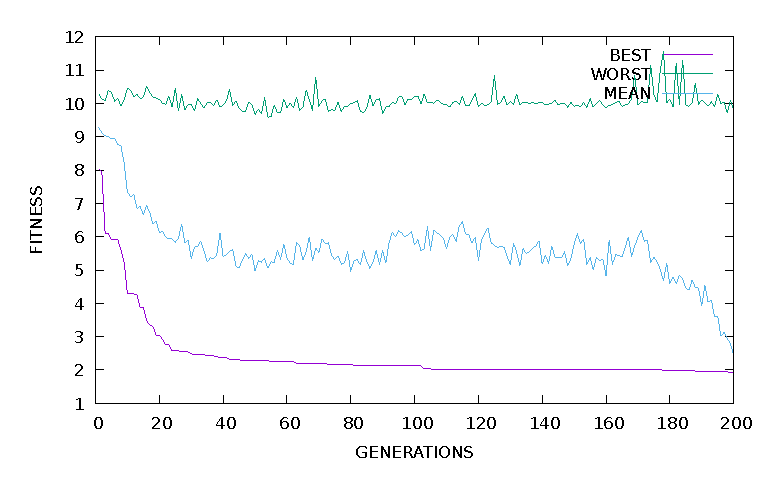
\includegraphics[scale=0.7]{wine_all_plot}
\end{figure}
\begin{figure}

\caption{Experiments with different values of $k$ for the Housing dataset.\label{fig:housing}}

\centering{}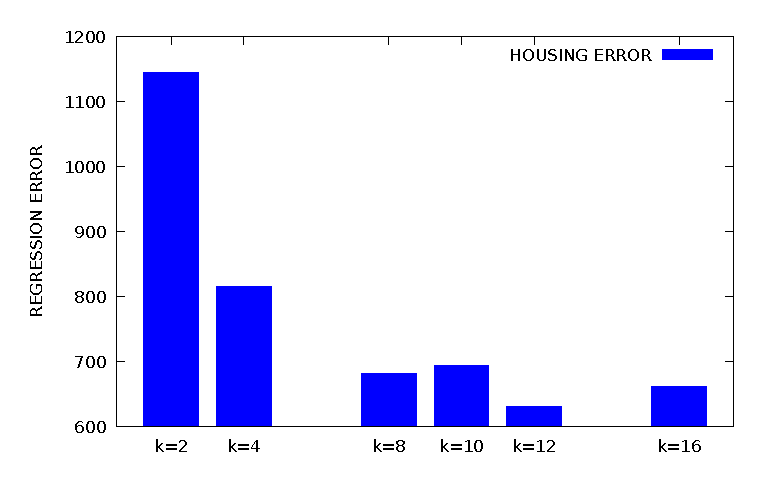
\includegraphics[scale=0.7]{housing}
\end{figure}
\begin{figure}
\caption{Classification error of Z\_F\_S dataset for different values of $k$.\label{fig:zfs}}

\centering{}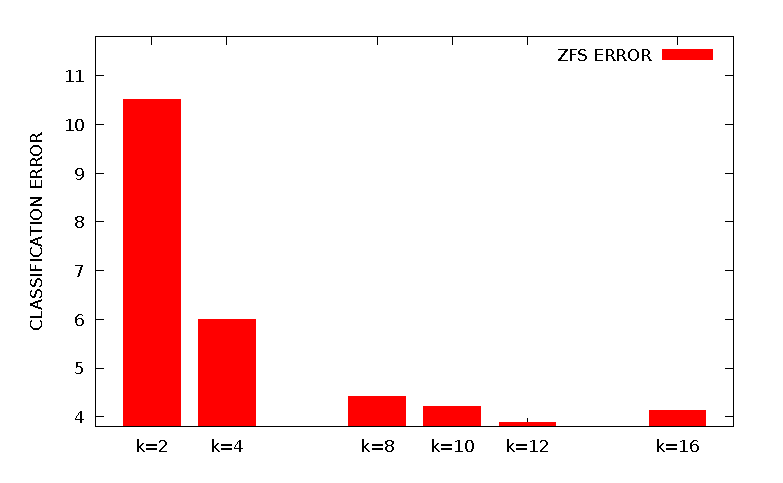
\includegraphics[scale=0.7]{zfs}
\end{figure}
\begin{table}

\caption{Comparison of precision and recall between the traditional RBF and
the proposed method for some datasets.\label{tab:Comparison-of-precision}}

\centering{}%
\begin{tabular}{|c|c|c|c|c|}
\hline 
DATASET & PRECISION KRBF & RECALL KRBF & PRECISION PROPOSED & RECALL PROPOSED\tabularnewline
\hline 
\hline 
HOUSEVOTES & 90.61\% & 95.60\% & 96.44\% & 94.25\%\tabularnewline
\hline 
SPIRAL & 55.53\% & 55.93\% & 82.93\% & 84.66\%\tabularnewline
\hline 
ZONF\_S & 92.76\% & 87.23\% & 97.27\% & 94.55\%\tabularnewline
\hline 
\end{tabular}
\end{table}


\section{Conclusions\label{sec:Conclusions}}

A two phase method was proposed in this article to train RBF neural
networks for classification and regression problems.\textbf{ }Firstly,
a common used clustering method was used to estimate an interval for
the critical parameters of the neural network. Subsequently, a parallel
genetic algorithm was incorporated to locate the best RBF network
with good generalization capabilities. The used software was coded
using ANSI C++ and open source libraries such as the Armadillo library
and the OpenMP library for parallelization. Future research may include
\begin{enumerate}
\item Use parallel methods for the k-means clustering phase of the method.
\item Dynamic selection of K in k-means algorithm. 
\item More advanced stopping rules for the genetic algorithm.
\item Replace the Genetic algorithm with other optimization methods such
as Particle Swarm Optimization, Ant Colony Optimization etc. 
\end{enumerate}

\subsection*{Acknowledgments}

The experiments of this research work was performed at the high performance
computing system established at Knowledge and Intelligent Computing
Laboratory, Dept of Informatics and Telecommunications, University
of Ioannina, acquired with the project \textquotedbl Educational
Laboratory equipment of TEI of Epirus\textquotedbl{} with MIS 5007094
funded by the Operational Programme \textquotedbl Epirus\textquotedbl{}
2014-2020, by ERDF and national finds.

\subsection*{Compliance with Ethical Standards }

All authors declare that they have no conflict of interest. 
\begin{thebibliography}{10}
\bibitem{rbf1}J. Park and I. W. Sandberg, Universal Approximation
Using Radial-Basis-Function Networks, Neural Computation 3, pp. 246-257,
1991.

\bibitem{ann-bishop}C.M. Bishop, Neural networks and their applications,
Review of Scientific Instruments \textbf{65}, pp. 1803-1832,1994.

\bibitem{rbfphysics1}P. Teng, Machine-learning quantum mechanics:
Solving quantum mechanics problems using radial basis function networks,
Phys. Rev. E \textbf{98}, 033305, 2018.

\bibitem{rbfphysics2}R. Jovanovi\'{c}, A. Sretenovic, Ensemble of
radial basis neural networks with K-means clustering for heating energy
consumption prediction, FME Transactions \textbf{45}, pp. 51-57, 2017.

\bibitem{rbfphysics3}A. Alexandridis, E. Chondrodima, E. Efthimiou,
G. Papadakis, F. Vallianatos and D. Triantis, Large Earthquake Occurrence
Estimation Based on Radial Basis Function Neural Networks,IEEE Transactions
on Geoscience and Remote Sensing \textbf{52}, pp. 5443-5453, 2014.

\bibitem{rbfphysics4}V.I. Gorbachenko, M.V. Zhukov, Solving boundary
value problems of mathematical physics using radial basis function
networks, Comput. Math. and Math. Phys. \textbf{57}, pp. 145--155,
2017. 

\bibitem{rbfmed1}Y.P. Wang, J.W. Dang, Q. Li and S. Li, Multimodal
medical image fusion using fuzzy radial basis function neural networks,
in 2007 International Conference on Wavelet Analysis and Pattern Recognition,
pp. 778-782, 2017.

\bibitem{rbfmed2}S, Mehrabi, M. Maghsoudloo, H. Arabalibeik, R. Noormand
and Y. Nozari, Congestive heart failure, Chronic obstructive pulmonary
disease, Clinical decision support system, Multilayer perceptron neural
network and radial basis function neural network, Expert Systems with
Applications \textbf{36}, pp. 6956-6959, 2009.

\bibitem{rbfmed3}M. Veezhinathan, S. Ramakrishnan, Detection of Obstructive
Respiratory Abnormality Using Flow--Volume Spirometry and Radial
Basis Function Neural Networks, J Med Syst \textbf{31}, pp. 461, 2007.

\bibitem{rbfde1}Nam Mai-Duy, Thanh Tran-Cong, Numerical solution
of differential equations using multiquadric radial basis function
networks, Neural Networks 14, pp. 185-199, 2001.

\bibitem{rbfde2}N. Mai-Duy, Solving high order ordinary differential
equations with radial basis function networks. Int. J. Numer. Meth.
Engng. \textbf{62}, pp. 824-852, 2005.

\bibitem{rbfchemistry1}Chuanhao Wan and Peter de B. Harrington, Self-Configuring
Radial Basis Function Neural Networks for Chemical Pattern Recognition,
J. Chem. Inf. Comput. Sci. \textbf{39}, 1049--1056, 1999.

\bibitem{rbfchemistry2}Xiaojun Yao, Xiaoyun Zhang, Ruisheng Zhang,
Mancang Liu, Zhide Hu, Botao Fan, Prediction of enthalpy of alkanes
by the use of radial basis function neural networks, Computers \&
Chemistry \textbf{25}, pp. 475-482, 2001.

\bibitem{rbfchemistry3}A. Shahsavand, A. Ahmadpour, Application of
optimal RBF neural networks for optimization and characterization
of porous materials, Computers \& Chemical Engineering 29, pp. 2134-2143,
2005.

\bibitem{rbfecon1}J. A. Momoh and S. S. Reddy, Combined Economic
and Emission Dispatch using Radial Basis Function, 2014 IEEE PES General
Meeting | Conference \& Exposition, National Harbor, MD, 2014, pp.
1-5, doi: 10.1109/PESGM.2014.6939506.

\bibitem{rbfecon2}Jau-Jia Guo and P. B. Luh, Selecting input factors
for clusters of Gaussian radial basis function networks to improve
market clearing price prediction, IEEE Transactions on Power Systems
\textbf{18}, pp. 665-672, 2003.

\bibitem{rbfecon3}L. Falat, Z. Stanikova, M. Durisova, B. Holkova,
T. Potkanova, Application of Neural Network Models in Modelling Economic
Time Series with Non-constant Volatility, Procedia Economics and Finance
\textbf{34}, pp. 600-607, 2015.

\bibitem{rbfnetwork1}C. Laoudias, P. Kemppi and C. G. Panayiotou,
Localization Using Radial Basis Function Networks and Signal Strength
Fingerprints in WLAN, GLOBECOM 2009 - 2009 IEEE Global Telecommunications
Conference, Honolulu, HI, 2009, pp. 1-6, 2009.

\bibitem{rbfnetwork2}S. Chen, B. Mulgrew and P. M. Grant, A clustering
technique for digital communications channel equalization using radial
basis function networks, IEEE Transactions on Neural Networks \textbf{4},
pp. 570-590, 1993.

\bibitem{rbf_add1}H. Jiang, Y. Yang, M. Shi, Chemometrics in Tandem
with Hyperspectral Imaging for Detecting Authentication of Raw and
Cooked Mutton Rolls, Foods \textbf{10}, 2021.

\bibitem{rbf_add2}H. Feng, Q. Song, S. Ma, W. Ma, C. Yin, D., H.
Yu, A new adaptive sliding mode controller based on the RBF neural
network for an electro-hydraulic servo system, ISA Transactions, 2022.

\bibitem{rbf_add3}X. Li, H. Jiang, X. Jiang, M. Shi, Identification
of Geographical Origin of Chinese Chestnuts Using Hyperspectral Imaging
with 1D-CNN Algorithm, Agriculture \textbf{11}, 2021.

\bibitem{rbf_add4}A.H. Fath, F. Madanifar, M. Abbasi, Implementation
of multilayer perceptron (MLP) and radial basis function (RBF) neural
networks to predict solution gas-oil ratio of crude oil systems, Petroleum
\textbf{6}, pp. 80-91, 2020.

\bibitem{rbf_add5}Y. Deng, X. Zhou, J. Shen, G. Xiao, H. Hong, H.
Lin, F. Wu, B.Q. Liao, New methods based on back propagation (BP)
and radial basis function (RBF) artificial neural networks (ANNs)
for predicting the occurrence of haloketones in tap water, Science
of The Total Environment \textbf{772}, 2021.

\bibitem{rbf_add6}H.R. Aqdam, M.M. Ettefagh, R. Hassannejad, Health
monitoring of mooring lines in floating structures using artificial
neural networks, Ocean Engineering \textbf{164}, Pages 284-297,2018.

\bibitem{rbfparallel}M.G. Arenas, E. Parras-Guti�rrez, V.M. Rivas,
P.A. Castillo, M.J. Del Jesus, J.J. Merelo. Parallelizing the Design
of Radial Basis Function Neural Networks by Means of Evolutionary
Meta-algorithms. In: Cabestany J., Sandoval F., Prieto A., Corchado
J.M. (eds) Bio-Inspired Systems: Computational and Ambient Intelligence.
IWANN 2009. Lecture Notes in Computer Science, vol 5517. Springer,
Berlin, Heidelberg, 2009.

\bibitem{rbfgpu}A. Brandstetter and A. Artusi, \textquotedbl Radial
Basis Function Networks GPU-Based Implementation,\textquotedbl{} in
IEEE Transactions on Neural Networks \textbf{19}, pp. 2150-2154, 2008.

\bibitem{rbfinit1}L.I. Kuncheva, Initializing of an RBF network by
a genetic algorithm, Neurocomputing \textbf{14}, pp. 273-288, 1997.

\bibitem{rbfinit2}M. Kubat, Decision trees can initialize radial-basis
function networks, IEEE Transactions on Neural Networks. \textbf{9},
pp. 813-821, 1998.

\bibitem{rbfinit3}D. G. B. Franco and M. T. A. Steiner, New Strategies
for Initialization and Training of Radial Basis Function Neural Networks,
IEEE Latin America Transactions.\textbf{ 15}, pp. 1182-1188, 2017.

\bibitem{rbfprun1}E. Ricci, R. Perfetti, Improved pruning strategy
for radial basis function networks with dynamic decay adjustment,
Neurocomputing \textbf{69}, pp. 1728-1732, 2006.

\bibitem{rbfprun2}M. Bortman and M. Aladjem, A Growing and Pruning
Method for Radial Basis Function Networks, IEEE Transactions on Neural
Networks \textbf{20}, pp. 1039-1045, 2009.

\bibitem{rbfprun3}Guang-Bin Huang, P. Saratchandran and N. Sundararajan,
A generalized growing and pruning RBF (GGAP-RBF) neural network for
function approximation, IEEE Transactions on Neural Networks \textbf{16},
pp. 57-67, 2005.

\bibitem{rbfpso1}J. Y. Chen, Z. Qin and J. Jia, A PSO-Based Subtractive
Clustering Technique for Designing RBF Neural Networks, 2008 IEEE
Congress on Evolutionary Computation (IEEE World Congress on Computational
Intelligence), Hong Kong, pp. 2047-2052, 2008.

\bibitem{rbfpso2}A. Esmaeili and N. Mozayani, Adjusting the parameters
of radial basis function networks using Particle Swarm Optimization,
2009 IEEE International Conference on Computational Intelligence for
Measurement Systems and Applications, Hong Kong, pp. 179-181, 2009.

\bibitem{rbfdiff1}B. O'Hora, J. Perera and A. Brabazon, Designing
Radial Basis Function Networks for Classification Using Differential
Evolution, The 2006 IEEE International Joint Conference on Neural
Network Proceedings, Vancouver, BC, pp. 2932-2937, 2006.

\bibitem{Tsoulos1}I.G. Tsoulos, Modifications of real code genetic
algorithm for global optimization, Applied Mathematics and Computation
\textbf{203}, pp. 598-607, 2008.

\bibitem{kmeans}MacQueen, J.: Some methods for classification and
analysis of multivariate observations, in: Proceedings of the fifth
Berkeley symposium on mathematical statistics and probability, Vol.
1, No. 14, pp. 281-297, 1967. 

\bibitem{kaeloali}P. Kaelo, M.M. Ali, Integrated crossover rules
in real coded genetic algorithms, European Journal of Operational
Research \textbf{176}, pp. 60-76, 2007.

\bibitem{Armadillo}C. Sanderson, R. Curtin, Armadillo: a template-based
C++ library for linear algebra, Journal of Open Source Software \textbf{1},
pp. 26, 2016. 

\bibitem{Keel}J. Alcal�-Fdez, A. Fernandez, J. Luengo, J. Derrac,
S. Garc�a, L. S�nchez, F. Herrera. KEEL Data-Mining Software Tool:
Data Set Repository, Integration of Algorithms and Experimental Analysis
Framework. Journal of Multiple-Valued Logic and Soft Computing 17,
pp. 255-287, 2011.

\bibitem{openmp}R. Chandra, L. Dagum, D. Kohr, D. Maydan,J. McDonald
and R. Menon, Parallel Programming in OpenMP, Morgan Kaufmann Publishers
Inc., 2001.

\bibitem{Alcohol}Tzimourta, Katerina D. and Tsoulos, Ioannis and
Bilero, Thanasis and Tzallas, Alexandros T. and Tsipouras, Markos
G. and Giannakeas, Nikolaos, Direct Assessment of Alcohol Consumption
in Mental State Using Brain Computer Interfaces and Grammatical Evolution,
Inventions \textbf{3}, pp. 1-12, 2018.

\bibitem{appendicitis}Weiss, Sholom M. and Kulikowski, Casimir A.,
Computer Systems That Learn: Classification and Prediction Methods
from Statistics, Neural Nets, Machine Learning, and Expert Systems,
Morgan Kaufmann Publishers Inc, 1991.

\bibitem{australian}J.R. Quinlan, Simplifying Decision Trees. International
Journal of Man-Machine Studies \textbf{27}, pp. 221-234, 1987. 

\bibitem{balance}T. Shultz, D. Mareschal, W. Schmidt, Modeling Cognitive
Development on Balance Scale Phenomena, Machine Learning \textbf{16},
pp. 59-88, 1994.

\bibitem{cleveland1}Z.H. Zhou,Y. Jiang, NeC4.5: neural ensemble based
C4.5,\textquotedbl{} in IEEE Transactions on Knowledge and Data Engineering
\textbf{16}, pp. 770-773, 2004.

\bibitem{cleveland2}R. Setiono , W.K. Leow, FERNN: An Algorithm for
Fast Extraction of Rules from Neural Networks, Applied Intelligence
\textbf{12}, pp. 15-25, 2000.

\bibitem{dermatology}G. Demiroz, H.A. Govenir, N. Ilter, Learning
Differential Diagnosis of Eryhemato-Squamous Diseases using Voting
Feature Intervals, Artificial Intelligence in Medicine. \textbf{13},
pp. 147--165, 1998.

\bibitem{glass1}G. Valentini, F. Masulli, NEURObjects: an object-oriented
library for neural network development, Neurocomputing \textbf{48},
pp. 623-646, 2002.

\bibitem{glass2}T. Denoeux, A neural network classifier based on
Dempster-Shafer theory, IEEE Transactions on Systems, Man and Cybernetics
- Part A: Systems and Humans \textbf{30}, pp. 131-150, 2000.

\bibitem{hayesroth}B. Hayes-Roth, B., F. Hayes-Roth. Concept learning
and the recognition and classification of exemplars. Journal of Verbal
Learning and Verbal Behavior \textbf{16}, pp. 321-338, 1977.

\bibitem{heart}I. Kononenko, E. �imec, M. Robnik-�ikonja, Overcoming
the Myopia of Inductive Learning Algorithms with RELIEFF, Applied
Intelligence \textbf{7}, pp. 39--55, 1997.

\bibitem{housevotes}R.M. French, N. Chater, Using noise to compute
error surfaces in connectionist networks: a novel means of reducing
catastrophic forgetting, Neural Comput. \textbf{14}, pp. 1755-1769,
2002.

\bibitem{ion1}J.G. Dy , C.E. Brodley, Feature Selection for Unsupervised
Learning, The Journal of Machine Learning Research \textbf{5}, pp
845--889, 2004.

\bibitem{ion2}S. J. Perantonis, V. Virvilis, Input Feature Extraction
for Multilayered Perceptrons Using Supervised Principal Component
Analysis, Neural Processing Letters \textbf{10}, pp 243--252, 1999.

\bibitem{liver} J. Garcke, M. Griebel, Classification with sparse
grids using simplicial basis functions, Intell. Data Anal. \textbf{6},
pp. 483-502, 2002.

\bibitem{mammographic}M. Elter, R. Schulz-Wendtland, T. Wittenberg,
The prediction of breast cancer biopsy outcomes using two CAD approaches
that both emphasize an intelligible decision process, Medical Physics
\textbf{34}, pp. 4164-4172, 2007

\bibitem{parkinsons}M.A. Little, P.E. McSharry, E.J. Hunter, J. Spielman,
L.O. Ramig, Suitability of dysphonia measurements for telemonitoring
of Parkinson's disease, IEEE Trans Biomed Eng. \textbf{56}, 2009.

\bibitem{pima}J.W. Smith, J.E. Everhart, W.C. Dickson, W.C. Knowler,
R.S. Johannes, Using the ADAP learning algorithm to forecast the onset
of diabetes mellitus, In: Proceedings of the Symposium on Computer
Applications and Medical Care IEEE Computer Society Press, pp.261-265,
1988.

\bibitem{popfailures}D.D. Lucas, R. Klein, J. Tannahill, D. Ivanova,
S. Brandon, D. Domyancic, Y. Zhang, Failure analysis of parameter-induced
simulation crashes in climate models, Geoscientific Model Development
\textbf{6}, pp. 1157-1171, 2013.

\bibitem{regions}N. Giannakeas, M.G. Tsipouras, A.T. Tzallas, K.
Kyriakidi, Z.E. Tsianou, P. Manousou, A. Hall, E.C. Karvounis, V.
Tsianos, E. Tsianos, A clustering based method for collagen proportional
area extraction in liver biopsy images, In: Proceedings of the Annual
International Conference of the IEEE Engineering in Medicine and Biology
Society, , pp. 3097-3100, 2015.

\bibitem{ring}B.L. Bias, variance and arcing classifiers. Tec. Report
460, Statistics department. University of california. April 1996. 

\bibitem{saheart}T. Hastie, R. Tibshirani, Non-parametric logistic
and proportional odds regression, JRSS-C (Applied Statistics) \textbf{36},
pp. 260--276, 1987.

\bibitem{segment}M. Dash, H. Liu, P. Scheuermann, K. L. Tan, Fast
hierarchical clustering and its validation, Data \& Knowledge Engineering
\textbf{44}, pp 109--138, 2003.

\bibitem{sonar}R.P. Gorman, T.J. Sejnowski, Analysis of Hidden Units
in a Layered Network Trained to Classify Sonar Targets, Neural Networks
\textbf{1}, pp. 75-89, 1988.

\bibitem{tae}T.S. Lim, W.Y. Loh, A Comparison of Prediction Accuracy,
Complexity, and Training Time of Thirty-Three Old and New Classification
Algorithms, Machine Learning \textbf{40}, pp. 203-228, 2000.

\bibitem{wdbc}W.H. Wolberg, O.L. Mangasarian, Multisurface method
of pattern separation for medical diagnosis applied to breast cytology,
Proc Natl Acad Sci U S A. \textbf{87}, pp. 9193--9196, 1990.

\bibitem{wine1}M. Raymer, T.E. Doom, L.A. Kuhn, W.F. Punch, Knowledge
discovery in medical and biological datasets using a hybrid Bayes
classifier/evolutionary algorithm. IEEE transactions on systems, man,
and cybernetics. Part B, Cybernetics : a publication of the IEEE Systems,
Man, and Cybernetics Society, \textbf{33} , pp. 802-813, 2003.

\bibitem{wine2}P. Zhong, M. Fukushima, Regularized nonsmooth Newton
method for multi-class support vector machines, Optimization Methods
and Software \textbf{22}, pp. 225-236, 2007.

\bibitem{zoo}M. Koivisto, K. Sood, Exact Bayesian Structure Discovery
in Bayesian Networks, The Journal of Machine Learning Research\textbf{
5}, pp. 549--573, 2004.

\bibitem{key-20}R.G. Andrzejak, K. Lehnertz, F. Mormann, C. Rieke,
P. David, and C. E. Elger, Indications of nonlinear deterministic
and finite-dimensional structures in time series of brain electrical
activity: Dependence on recording region and brain state, Phys. Rev.
E \textbf{64}, pp. 1-8, 2001.

\bibitem{abalone}W. J Nash, T.L. Sellers, S.R. Talbot, A.J. Cawthor,
W.B. Ford, The Population Biology of Abalone (\_Haliotis\_ species)
in Tasmania. I. Blacklip Abalone (\_H. rubra\_) from the North Coast
and Islands of Bass Strait, Sea Fisheries Division, Technical Report
No. 48 (ISSN 1034-3288), 1994.

\bibitem{airfoil}T.F. Brooks, D.S. Pope, and A.M. Marcolini. Airfoil
self-noise and prediction. Technical report, NASA RP-1218, July 1989. 

\bibitem{anacalt} Jeffrey S. Simonoff, Analyzing Categorical Data,
Springer-Verlag, New York, 2003.

\bibitem{concrete}I.Cheng Yeh, Modeling of strength of high performance
concrete using artificial neural networks, Cement and Concrete Research.
\textbf{28}, pp. 1797-1808, 1998. 

\bibitem{key23}D. Harrison and D.L. Rubinfeld, Hedonic prices and
the demand for clean ai, J. Environ. Economics \& Management \textbf{5},
pp. 81-102, 1978.

\bibitem{key21}J.S. Simonoff, Smooting Methods in Statistics, Springer
- Verlag, 1996.

\bibitem{thyroid}Quinlan,J.R., Compton,P.J., Horn,K.A., and Lazurus,L.
(1986). Inductive knowledge acquisition: A case study. In Proceedings
of the Second Australian Conference on Applications of Expert Systems.
Sydney, Australia.

\bibitem{ntdataset}Mackowiak, P.A., Wasserman, S.S., Levine, M.M.,
1992. A critical appraisal of 98.6 degrees f, the upper limit of the
normal body temperature, and other legacies of Carl Reinhold August
Wunderlich. J. Amer. Med. Assoc. 268, 1578--1580

\bibitem{Stat}J.S. Simonoff, Smooting Methods in Statistics, Springer
- Verlag, 1996.

\bibitem{rbf_gen1}S. Ding, L. Xu, C. Su et al, An optimizing method
of RBF neural network based on genetic algorithm. Neural Comput \&
Applic 21, pp. 333--336, 2012.
\end{thebibliography}

\end{document}
